\documentclass{article}
    \usepackage[utf8]{inputenc}

    \title{Serial Code Optimisation}
    \author{David Sharp:ds16797 Candidate 36688}
    \date{October 2018}
    \usepackage[legalpaper, portrait, margin=1.5cm]{geometry}
    \usepackage{amsmath}
    \usepackage{graphicx}
    \usepackage{float}
    
    \begin{document}

    \maketitle
    \section{Introduction}
    In summary, I managed to partially optimise the 5-point stencil but not to the benchmarks listed in the assignment.
    In this report I will detail the optimisation techniques that worked for me and also outline the optimisations I hoped to utilise
    but couldn't fully implement.
    \section{Optimisations}
    \subsection{Initial State}
    \begin{center}
    \begin{tabular}{| c | c | c | c |}
    Compiler settings & 1024 image/s & 4096 image/s & 8000 image/s \\ \hline
    No flags gcc4.8.4 & 8.23 & 318 & 735 \\
    No flags gcc7.1.0 & 8.20 & 433 & 577 \\
    -O3 gcc7.1.0 & 6.81 & 121 & 362 \\
    -Ofast gcc7.1.0 & 2.34 & 108 & 125 \\
    No flags icc16 & 3.40 & 49.3 & 176 \\
    -xHost icc16 & 3.42 & 49.3 & 175 \\
    -Ofast icc16 & 2.13 & 93.6 & 105
    \end{tabular}
    \end{center}
    These initial optimisations (visualised in Figure 1) already show some interesting results, with gcc7.1.0 not being consistently faster across different scales and the Intel
    compiler icc version 16 being significantly faster than gcc7.1.0.
    -O3 and -Ofast each gave significant speedups on gcc, while -xHost - designed to adapt the code for the specific Intel processor - offered no speedup
    over the icc defaults.
    
    \subsection{Profiling}
    After getting the initial simple speedup from compiler flags, I ran gprof to get an intuition for where the majority of the runtime is located.
    The results were as following on the 1024 image.
    \begin{center}
    \begin{tabular}{| c | c | c | c |}
    Percentage Time & Self Seconds & Calls & Name \\ \hline
    99.84 & 8.19 & 200 & stencil \\
    0.37 & 0.03 & 1 & init\_image \\
    0.12 & 0.01 & 1 & output\_image \\
    0.00 & 0.00 & 2 & wtime
    \end{tabular}
    \end{center}
    Data from the gprof profiling. It's very clear that the $stencil$ function is the limiter on the code speed, since it is run 200 times. As such
    it makes the most sense to focus optimisation on this one function.
    \subsection{Code Optimisation}
    My first thought for optimising the code was to reduce the math operation for each part of the stencil, changing the value change by multiplication 
    then division by simplifying into a single multiplication. While this change may be already carried out by the more rigorous compiler flags, it makes
    the code more readable and from my own research multiplication is at least as fast as division in many languages.
    Following this I tried swapping the values of $i$ and $j$ to hopefully achieve better ordering; in the course of which I realised that I could try
    accessing the image array with some single variable $z$ allowing me to use a single loop and potentially achieve better vectorisation since there would
    no longer be any nesting.
    Through math changes and compiler flags as listed above the small image was computing in about 1.37 seconds. It was at this point that I decided it would
    be worthwhile to run a vectorisation report with gcc to get an idea of what was limiting the vectorisation.
    From gcc's vectorisation report I found out that as I had expected, the nesting of loops was a major reason why the code was not vectorising, followed
    by conditionals/branching within loops. I remembered from lecture content that restricting pointers might also help with vectorisation and other optimisation,
    since $tmp\_image$ and $image$ are wholly separate lists, there was no danger in stating in $stencil$ that they were restricted pointers and didn't access any
    of the same memory space. This change led to the code running in $1/3$ the time, 0.441 seconds.
    \subsection{Failed Optimisations}
    At this point I tried first swapping to a single for loop structure within $stencil$, however that change alone made no difference to the runtime - I imagine
    since no additional vectorisation could occur since the conditionals were still in $stencil$ - and worse yet, I couldn't manage to implement in such a way that
    it would work correctly, the python script would always fail.
    Then I split up computation into several discrete for loops, two for the top and bottom row edge cases and two for the left and right column edge cases, with
    each corner of the grid being computed outside of any loop. This allowed me to remove most conditionals from the main for loop body, though I still needed
    to check when $z$ in the main for loop hit the rightmost column so I could increase it to skip the left and right edge cases.
    After implementing these changes the code ran in nearly $1/2$ the time that I had reached before, 0.253 seconds - I imagine due to a higher level of vectorisation
    since I had removed the conditionals and nested nested loops - unfortunately this code too did not pass the python script.
    I reverted my changes back to the last correct code commit and tried swapping $double$ data types for $float$, which in theory should allow more of the 
    image data to fit in cache at once, reduce the amount of cache misses and thereby reduce the amount of cycles used on accessing higher levels of cache or DRAM.
    However when I made the change and tested it the runtime got longer, 2x the runtime for the 1024 image up to nearly 3x the runtime for the 8000 image on gcc, with
    icc not being quite as bad on the large image (about 2x normal icc runtime).
    This seems like quite a surprising result, I imagine perhaps there is more hardware optimisation for doubles
    \subsection{End Results}
    It was at this point that I found my most interesting result, I tested different compilers again to see if icc could still offer some performance increase like
    it had when the code was fully unoptimised. As seen below, icc16 was slower across all image sizes perhaps due to differing optimisations and maybe not helped
    by the fact that I used gcc during my development meaning that perhaps some changes that I made would have been better suited to icc but I would never know.
    It seems clear that the code is memory bound, particularly for medium and large images, the algorithm has approximate complexity $O(n^2)$ and so the 4096 image
    should run in about 16x the runtime of the 1024 and the 8000 image should run in about 4x the runtime of the 4096. From these estimates there is clearly some
    slowdown in the larger images and I think this is due to more time relatively spent accessing memory.
    The greatest issue with my optimisation is that very limited vectorisation occurs so I am not very close to the computational limit even if my memory bandwidth were to be perfect, which I doubt. 
    
    \begin{center}
    \begin{tabular}{| c | c | c | c |}
    Compiler & 1024 image/s & 4096 image/s & 8000 image/s \\ \hline
    gcc7.1.0 -Ofast & 0.441 & 7.58 & 30.2 \\
    icc16 -Ofast & 0.542 & 9.38 & 35.6 
    \end{tabular}
    \end {center}
    
    \section{Conclusion}
    Overall I believe it was the implementation, not the optimisation approach that meant I didn't hit the benchmarks; the tests I ran on separating the edge cases
    from the main for loop body and removing nesting led to runtimes within the listed benchmarks but the python script failed on many of the image elements. I tried
    using different approaches to achieve the same result, namely using a halo of zeroed cells around the outside so that the entire image could be run without 
    conditionals within a single for loop, but in this case the python script failed to run at all - likely because I was messing with the dimensions of $image$ and
    $tmp\_image$.
    Some of the results were very surprising to me; as a result optimisation seems both more understandable and more unpredictable. I didn't expect to see such a large difference between compilers at the beginning of the coursework only to see a smaller difference in the other direction once I had finished. I also didn't expect
    such a drastic difference between $float$ and $double$ and between $value*3.0/5.0$ and $value*0.6$.
    I think the most useful thing that I have learned from the coursework has been the tools to get started on optimising code e.g profiling,vectorisation reports, 
    compiler flags and the understanding that it has to be a testing driven process. With all the inbuilt compiler optimisations, I've learned there is no point in
    just diving straight in and trying to change every bit of code since there is a good chance the compiler has already done it.
    
    \begin{figure}[H]
    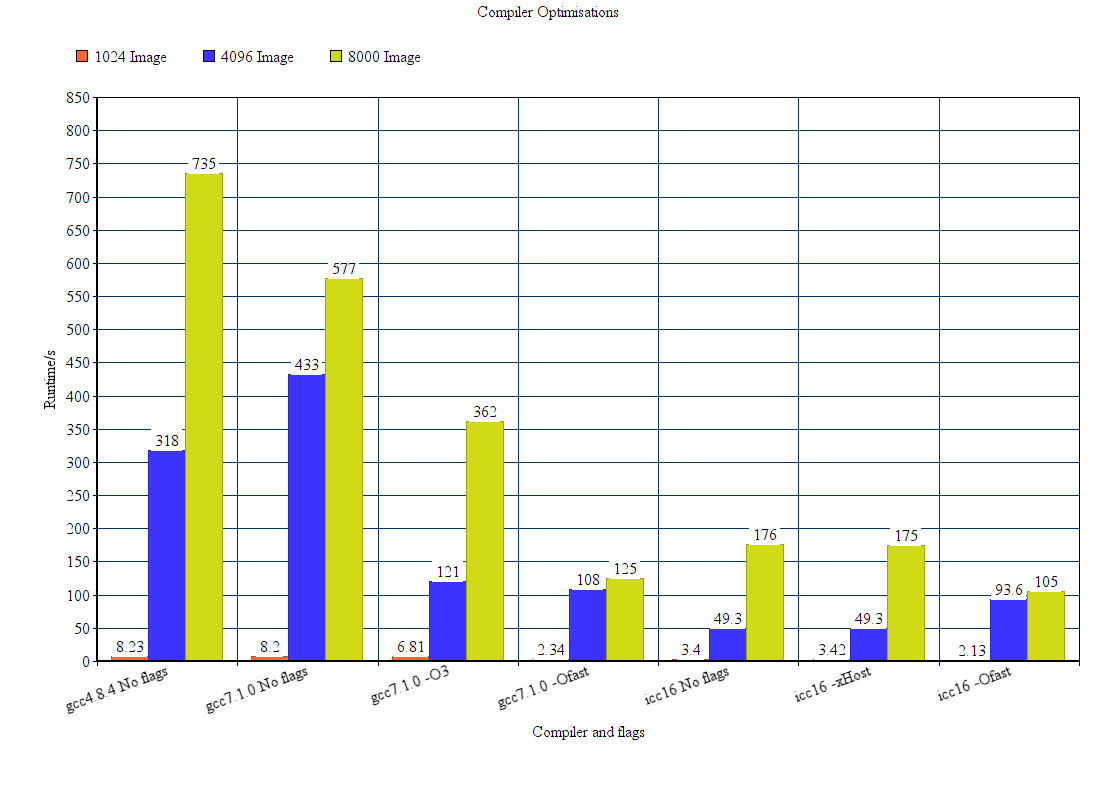
\includegraphics[scale=0.5]{graph.png}
    \label{fig:graph}
    \caption{Compiler Optimisation Bar Graph}
    \end{figure}
    \end{document}